\begin{equation*}
% the lanes take the site's --mred (#7a2518); the link boxes are white-outlined, filled with the ink's complement
\definecolor{lanecolor}{RGB}{122,37,24}\colorlet{paper}{-.}%
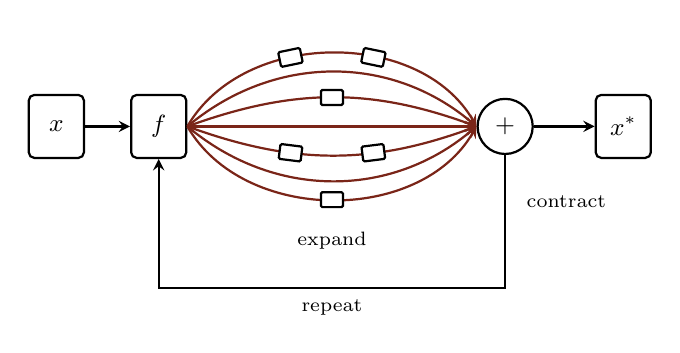
\begin{tikzpicture}[
  inst/.style={draw, rounded corners=2pt, thick, minimum width=7mm, minimum height=8mm, font=\small},
  fold/.style={draw, circle, thick, minimum size=7mm, font=\small},
  hop/.style={thick, ->, >=stealth},
  lane/.style={thick, ->, >=stealth, color=lanecolor},
  link/.style={draw, fill=paper, thick, rounded corners=0.5pt, minimum width=2.8mm,
               minimum height=1.9mm, inner sep=0pt},
  note/.style={font=\scriptsize}
]
\node[inst] (x) at (0,0)   {$x$};
\node[inst] (f) at (1.3,0) {$f$};
\draw[hop] (x) -- (f);
\node[fold] (m) at (5.7,0) {$+$};
\foreach \ang in {-60,-40,-20,0,20,40,60}
  \draw[lane] (f.east) to[bend left=\ang] (m.west);
\path (f.east) to[bend left=60] node[link, pos=0.38, sloped] {} node[link, pos=0.62, sloped] {} (m.west);
\path (f.east) to[bend left=20] node[link, pos=0.5, sloped] {} (m.west);
\path (f.east) to[bend left=-20] node[link, pos=0.35, sloped] {} node[link, pos=0.65, sloped] {} (m.west);
\path (f.east) to[bend left=-60] node[link, pos=0.5, sloped] {} (m.west);
\node[inst] (xs) at (7.2,0) {$x^{*}$};
\draw[hop] (m) -- (xs);
% the back edge: the frontier one pass leaves is the next pass's
\draw[hop] (m.south) -- (5.7,-2.05) -- (1.3,-2.05) -- (f.south);
\node[note] at (3.5,-1.45) {expand};
\node[note, anchor=west] at (5.85,-0.95) {contract};
\node[note] at (3.5,-2.3) {repeat};
\end{tikzpicture}
\end{equation*}
